%\pagestyle{plain}

\chapter{Related work}\label{chap:related work}

Nowadays, neural networks are widely used in the field of image processing, pattern recognition, human movement analysis and many more. There are numerous types of tasks concerning human movement analysis, where the neural networks proved to be beneficial, e.g. action recognition, action classification, body-movement-based human identification, pose estimation etc.\par
\vspace{5mm}
\noindent Focusing on the pose estimation task, there have been many different methods and approaches presented in recent years. Based on the type of the input data, the studies can be divided into approaches inferring from two-dimensional data (RGB images) and three-dimensional data (depth maps, point clouds, voxelized grids etc.). The two-dimensional approaches are far more usable and easily accessible in real-time applications, being able to run without any special devices, using only the RGB camera. On the other hand, the regression of 3D joint positions from 2D input data requires highly non-linear operations, what can lead to many difficulties in the learning procedure. The three-dimensional approaches provide the additional depth information, which can significantly simplify the task for the network, and thus improve the estimation accuracy.

\section{Two-dimensional input data}
\noindent Among studies working with the RGB data, Mehta et al. \cite{VNect_SIGGRAPH2017} introduced a system called \textit{VNect} to obtain real-time full global 3D skeletal pose, combining a pose regressor based on convolutional neural network with kinematic skeleton fitting. They also invented a new concept of the so-called \textit{location maps}, that are produced by the network, along with the confidence heatmaps for each joint. The network outputs three location maps and one heatmap per joint. The predicted 3D position of each body joint is read out from three location maps, corresponding to x, y, and z coordinate, at the estimated pixel location of the particular keypoint, determined by the heatmap. The pipeline introduced in the stated paper is shown in Fig. \ref{fig:Vnect}.\par

\vspace{5mm}
\begin{figure}[H]
\begin{center}
  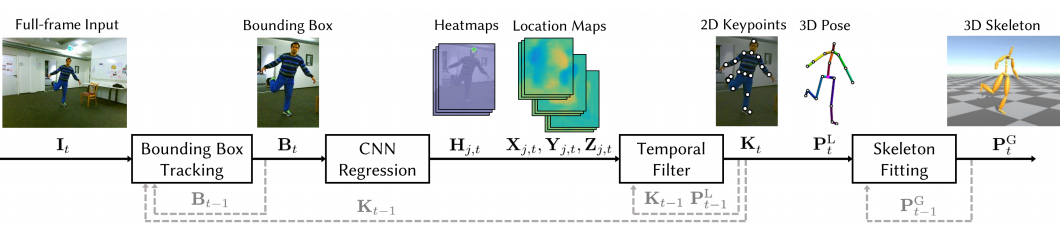
\includegraphics[width=\textwidth]{images/related_work/VNect.PNG}
  \caption{The overview of the VNect pipeline \cite{VNect_SIGGRAPH2017}.}
  \label{fig:Vnect}
\end{center}
\end{figure}

\noindent However, the stated model was unable to handle occlusions or capture multiple people in the scene. Thus, they removed these restrictions in the follow-up model called \textit{XNect} \cite{DBLP:journals/corr/abs-1907-00837}, which is able to capture multiple people in the scene by a single RGB camera. Unlike the previous work, the model outputs full skeletal pose in joint angles and global body positions of a coherent skeleton in real-time. The method consists of three subsequent stages: First, a convolutional neural network estimates 2D and 3D features and identity assignments for all visible body joints of all subjects in the scene, second, a fully-connected neural network turns possibly occluded 2D and 3D pose features into a complete 3D pose per subject, and third, a space-time skeletal model fitting is applied to the predicted 2D and 3D pose to merge them and enforce temporal coherence.\par
\vspace{5mm}
\noindent
In another paper, Mehta et al. \cite{mono-3dhp2017} focused on RGB data as well, but this time, they presented a method based on the concept of transfer learning. They embraced the similarity between the feature extraction tasks in 2D and 3D space, and transferred the features learned on 2D data to 3D pose estimation network (that is, pre-trained the 3D convolutional model on 2D features). In the paper, they put a great emphasis on \textit{in-the-wild} scenes, that is, the pipeline was designed to perform well even outside of the recording room, in generic outdoor scenes. Newell \cite{DBLP:journals/corr/NewellYD16} presented stacked hourglass networks, consisting of multiple stacked hourglass modules which allow for repeated bottom-up, top-down inference. These networks are designed such that the features are processed across all scales, allowing them to capture the spatial relationships within the body. Chou et al. \cite{DBLP:journals/corr/ChouCC17} employed generative adversarial networks as the learning paradigm. They consist of two stacked hourglass networks – generator and discriminator, where the former is used for the human pose estimation and the latter back-propagates the adversarial loss between the ground-truth and the generated output to the generator. \par
\vspace{5mm}
\noindent
Rogez et al. \cite{lcrnet} decided to utilize the concept of the pre-defined anchor poses. Their proposed pipeline consists of three sub-tasks. First, they extract candidate regions using a Region Proposal Network \cite{NIPS2015_5638} and place the set of anchor poses into the predicted bounding boxes. Then, they run it through a classification branch, which outputs probabilities of anchor poses to be correct at each location. Finally, the regression branch computes an anchor-pose-specific regression that estimates the difference between the pose proposal and ground-truth pose, and refines the final pose estimation. 

\section{Three-dimensional input data}
\noindent The three-dimensional data used as the input to the neural networks come in various forms. Most frequently, 3D input data are in a form of depth maps (RGB-D images). Depth maps are actually encoding 3D space into 2D image, where the value at each pixel position represents the corresponding depth value (third axis coordinate). Marin-Jimenez et al. \cite{Marin18jvcir} proposed a technique where the final estimated pose is computed as the weighted sum of the predefined set of prototype poses. The weights corresponding to the prototypes are directly regressed from input depth maps by a convolutional neural network. In the paper, they claim to have outperformed state-of-the-art results on the benchmark datasets and reached 100\% accuracy in mean average precision at 10cm on the ITOP dataset \cite{haque2016viewpoint}, i.e. every skeleton joint is predicted within 10cm range from its ground-truth position. The stated approach is an example of a single-stage method.\par
\vspace{5mm}
\noindent The two-stage methods generally consists of the segmentation stage and the regression stage. First, the input data is segmented to the corresponding body-parts. Then, the segmented input data is used to infer 3D joint coordinates. An example of a two-stage method was proposed by Shafaei and Little \cite{Shafaei16}. They treat the problem of 3D pose estimation from depth data through two-stage pipeline, where in the first stage the body parts are identified from the input depth maps by a dense classifier. In the second stage, all camera views are merged, and the created unified 3D point cloud is passed to a linear regressor to compute 3D body joint locations. \par
\vspace{5mm}
\noindent Aside from depth maps, some of the methods make use of the voxelized grids, made by discretizing a given point cloud in a predefined set of values. However, voxels require use of three-dimensional convolutions, what makes working with them very time-consuming and computationally expensive. \textit{V2V PoseNet} \cite{DBLP:journals/corr/abs-1711-07399} operates with this kind of data and regresses joint locations with 3D CNN-autoencoders. They first use 3D CNN encoder and decoder to estimate per-voxel likelihood of each skeleton joint from voxelized input (Fig. \ref{fig:v2vposenet}). Afterwards, they refine the target object localization with a 2D CNN which takes a cropped depth map and output an offset from the its reference point to the center of ground truth joint positions. This way, they obtain an accurate reference point.\par

\vspace{5mm}
\begin{figure}[H]
\begin{center}
  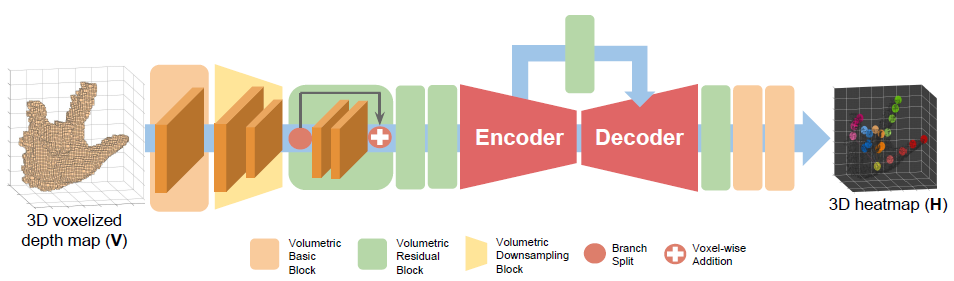
\includegraphics[width=\textwidth]{images/related_work/v2vposenet.PNG}
  \caption[The V2V-PoseNet architecture \cite{DBLP:journals/corr/abs-1711-07399}.]{The V2V-PoseNet architecture which takes voxelized input and estimates the per-voxel likelihood for each keypoint \cite{DBLP:journals/corr/abs-1711-07399}.}
  \label{fig:v2vposenet}
\end{center}
\end{figure}



\noindent Nevertheless, there are several networks proposed which work with unordered point clouds as input data, yet implement the convolution operations on the point clouds without using computationally expensive 3D convolutions. Some of the methods decided to use shared multi-layered perceptrons and max-pooling layers to obtain the features of point cloud. Although they extract global features, since the max-pooling layers are applied on the whole set of points, it is hard to capture local features.\par
\vspace{5mm}


\noindent Qi et al. \cite{DBLP:journals/corr/QiSMG16} proposed a classification and segmentation model called \textit{PointNet}, where they intended to incorporate the local features by aggregation of the intermediate outputs from the classification network, before and after max-pooling. Afterwards, they fed the aggregated local and global features into the segmentation network. Later, Qi et al. \cite{DBLP:journals/corr/QiYSG17} introduced \textit{PointNet++} model, which has similar key structure as the previous PointNet, but improves the model by utilizing a hierarchical structure, similar to the one used in image convolutional neural networks. It recursively applies PointNet on a nested partitioning of input point cloud, starting from small local regions and gradually extending to bigger regions. The whole hierarchical feature learning architecture (on 2D point set example) suggested in the paper is shown in Fig. \ref{fig:Pointnet2}. \par

\vspace{5mm}

\noindent In another study, Wu et al. \cite{DBLP:journals/corr/abs-1811-07246} presented a new convolution operation called \textit{PointConv}, which can be applied on unordered and irregular point clouds. They treat convolution kernels as nonlinear weight and density functions of the local coordinates of 3D points. The weight functions are learned with multi-layer perceptron networks and density functions through kernel density estimation. Such learned kernels can be used for translation-invariant and permutation-invariant convolutions on any 3D point set. \par
\vspace{5mm}
\begin{figure}[H]
\begin{center}
  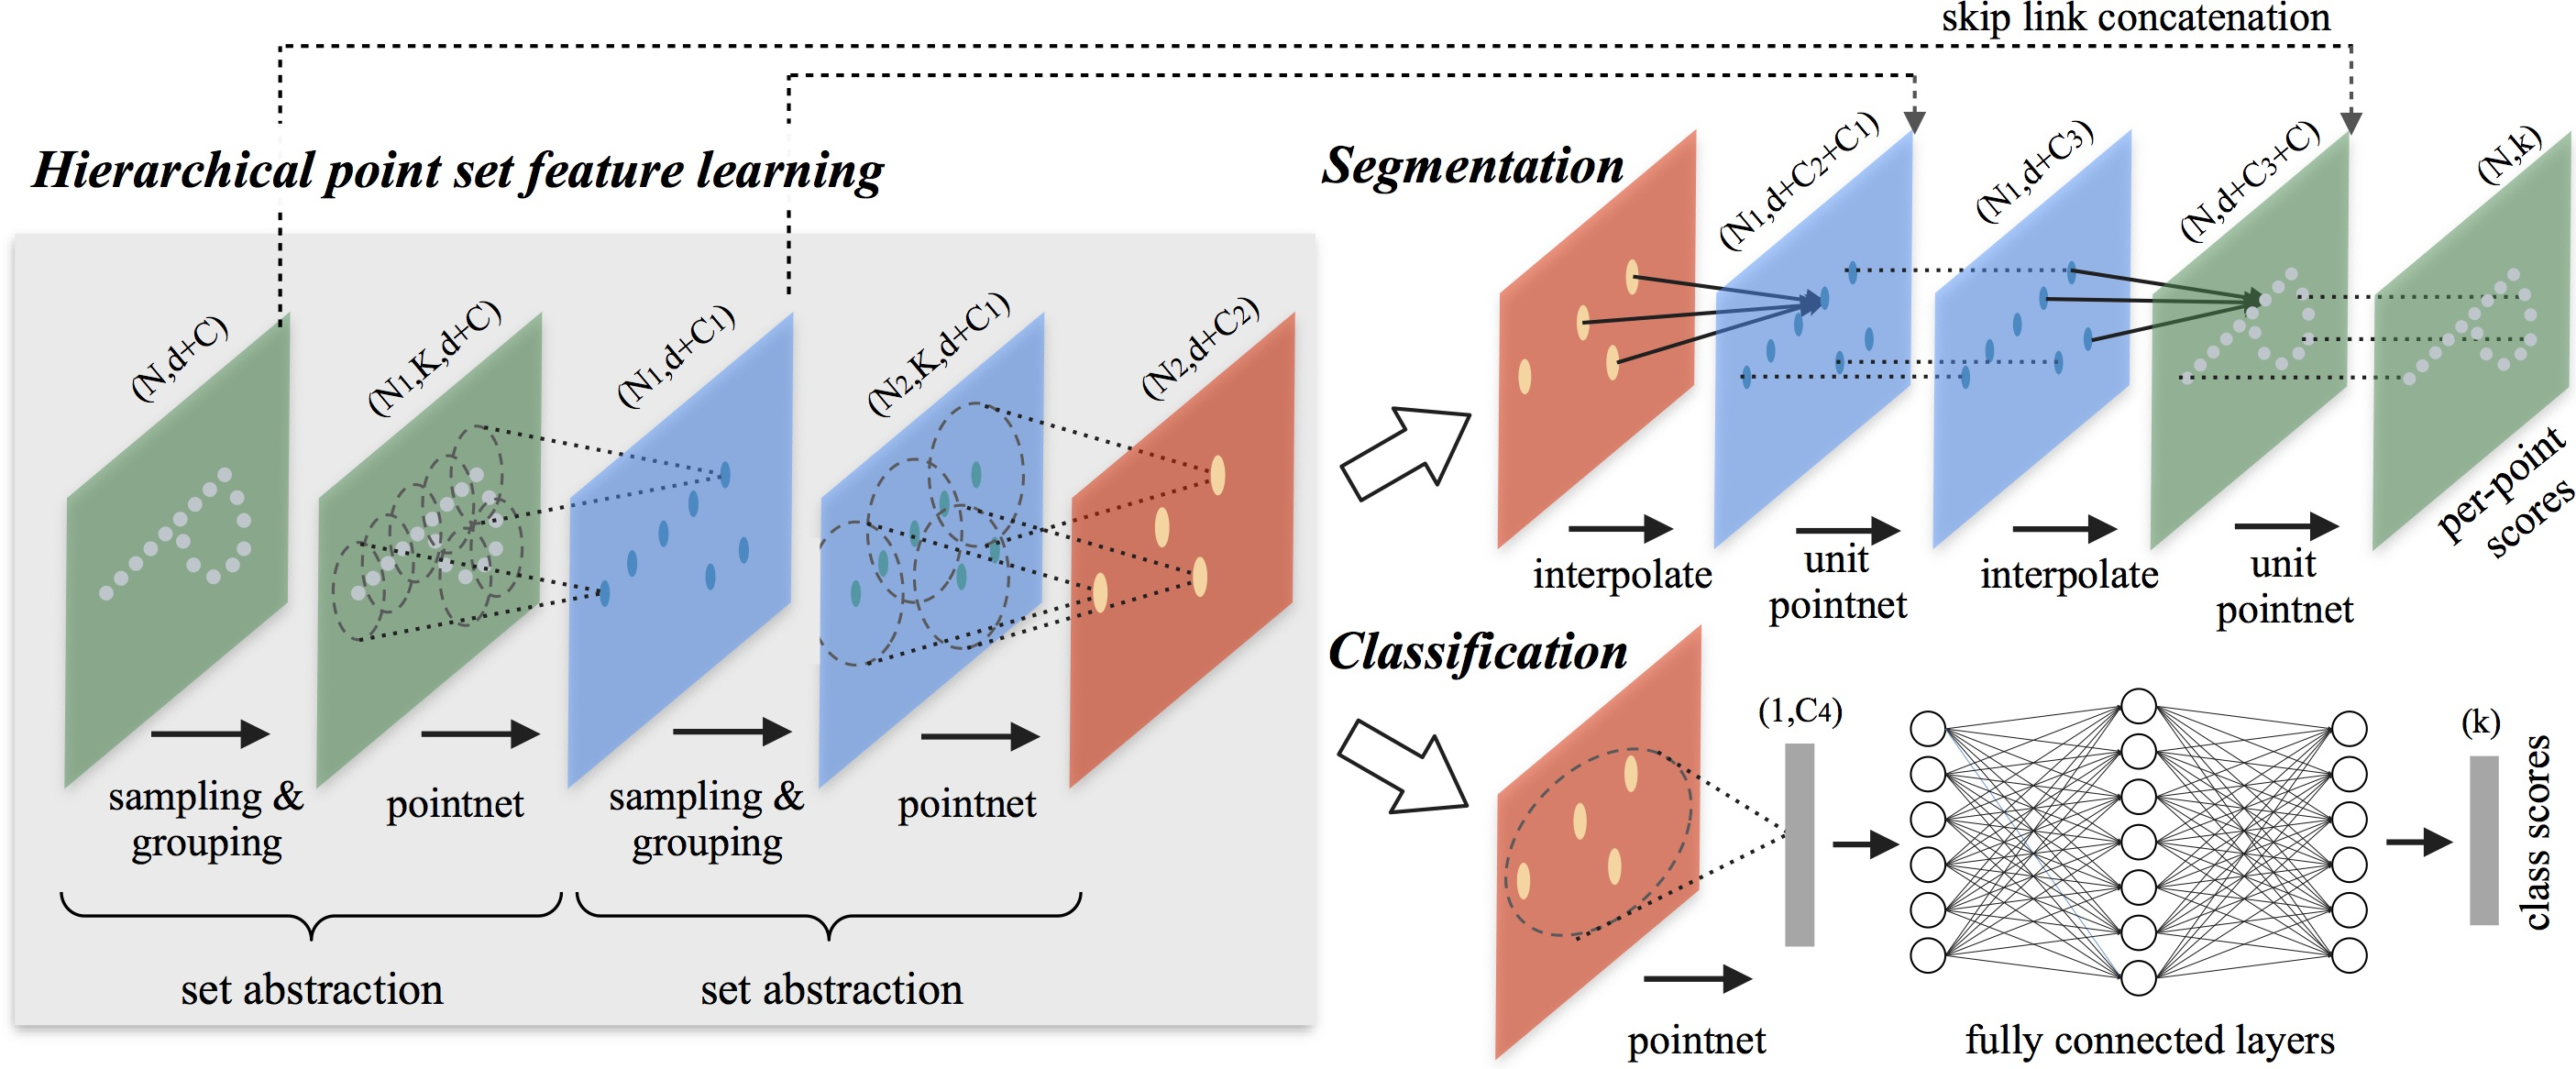
\includegraphics[width=\textwidth]{images/related_work/pointnet2.jpg}
  \caption[The PointNet++ hierarchical feature learning architecture \cite{DBLP:journals/corr/QiYSG17}.]{The PointNet++ hierarchical feature learning architecture shown on points from 2D Euclidean space \cite{DBLP:journals/corr/QiYSG17}.}
  \label{fig:Pointnet2}
\end{center}
\end{figure}

\noindent It is worth mentioning, that all of the stated methods processing unordered point clouds perform object classification or segmentation task, which is not an aim of our thesis. Concerning pose estimation task, Ali \cite{Ali19} introduced a novel one-stage approach in his thesis called \textit{Point-Based Pose Estimation} (PBPE), taking point clouds directly as input data to the model which outputs 3D skeleton joint coordinates. He concludes, that since point clouds are able to provide sparser representation of the human body than depth maps, the operations on them would be much easier, and thus, the computational complexity would be reduced. The inspiration for the model was in the PointNet architecture. Besides the proposed PBPE model, the contribution of his work also consists of the refinement of several two-stage methods by using an automatic annotation mechanism for labeling body regions in real data. Next, the study presents the benefits of fusion of the real training data and more complex synthetic training data. The poses in the synthetic dataset are much more varied, so by adding certain amount of the synthetic data to the real dataset during the training phase, they extend the diversity of the training set. As a result, the model is able to generalize better. On the other hand, the synthetic data is also useful for pre-training a model, reducing the computational cost and time of the real data annotation. Thus, such pre-trained model can be fine-tuned on relatively small part of the real dataset, yet achieving reasonable results. \par

% + pridat nejake obrazky ==> viac stran


% + pri MHAD datasete spomenut nizku presnost ground truth labelov (Kinect360) - povodne primarne urceny na action recognition (tam nizka presnost nemusi az tak prekazat), pri ITOP datasete pomerne maly rozsah, pri UBC sice synteticke data - bez sumu, vzdialenejsie realnym, ale presne ground truth labels ==> vlastny dataset idealne/PKUMMD (Kinect v2), spomenut nedostatok large depth data pose estimation datasetov verejne dostupnych



%\begin{equation}
%	\frac{1}{r_{B}} = \frac{1}{r_{A}} + \frac{1}{r_{C}},
%\end{equation}


